\section{Model of Feedback}\label{sec:feedback-model}

\begin{figure}[htb]
\centering
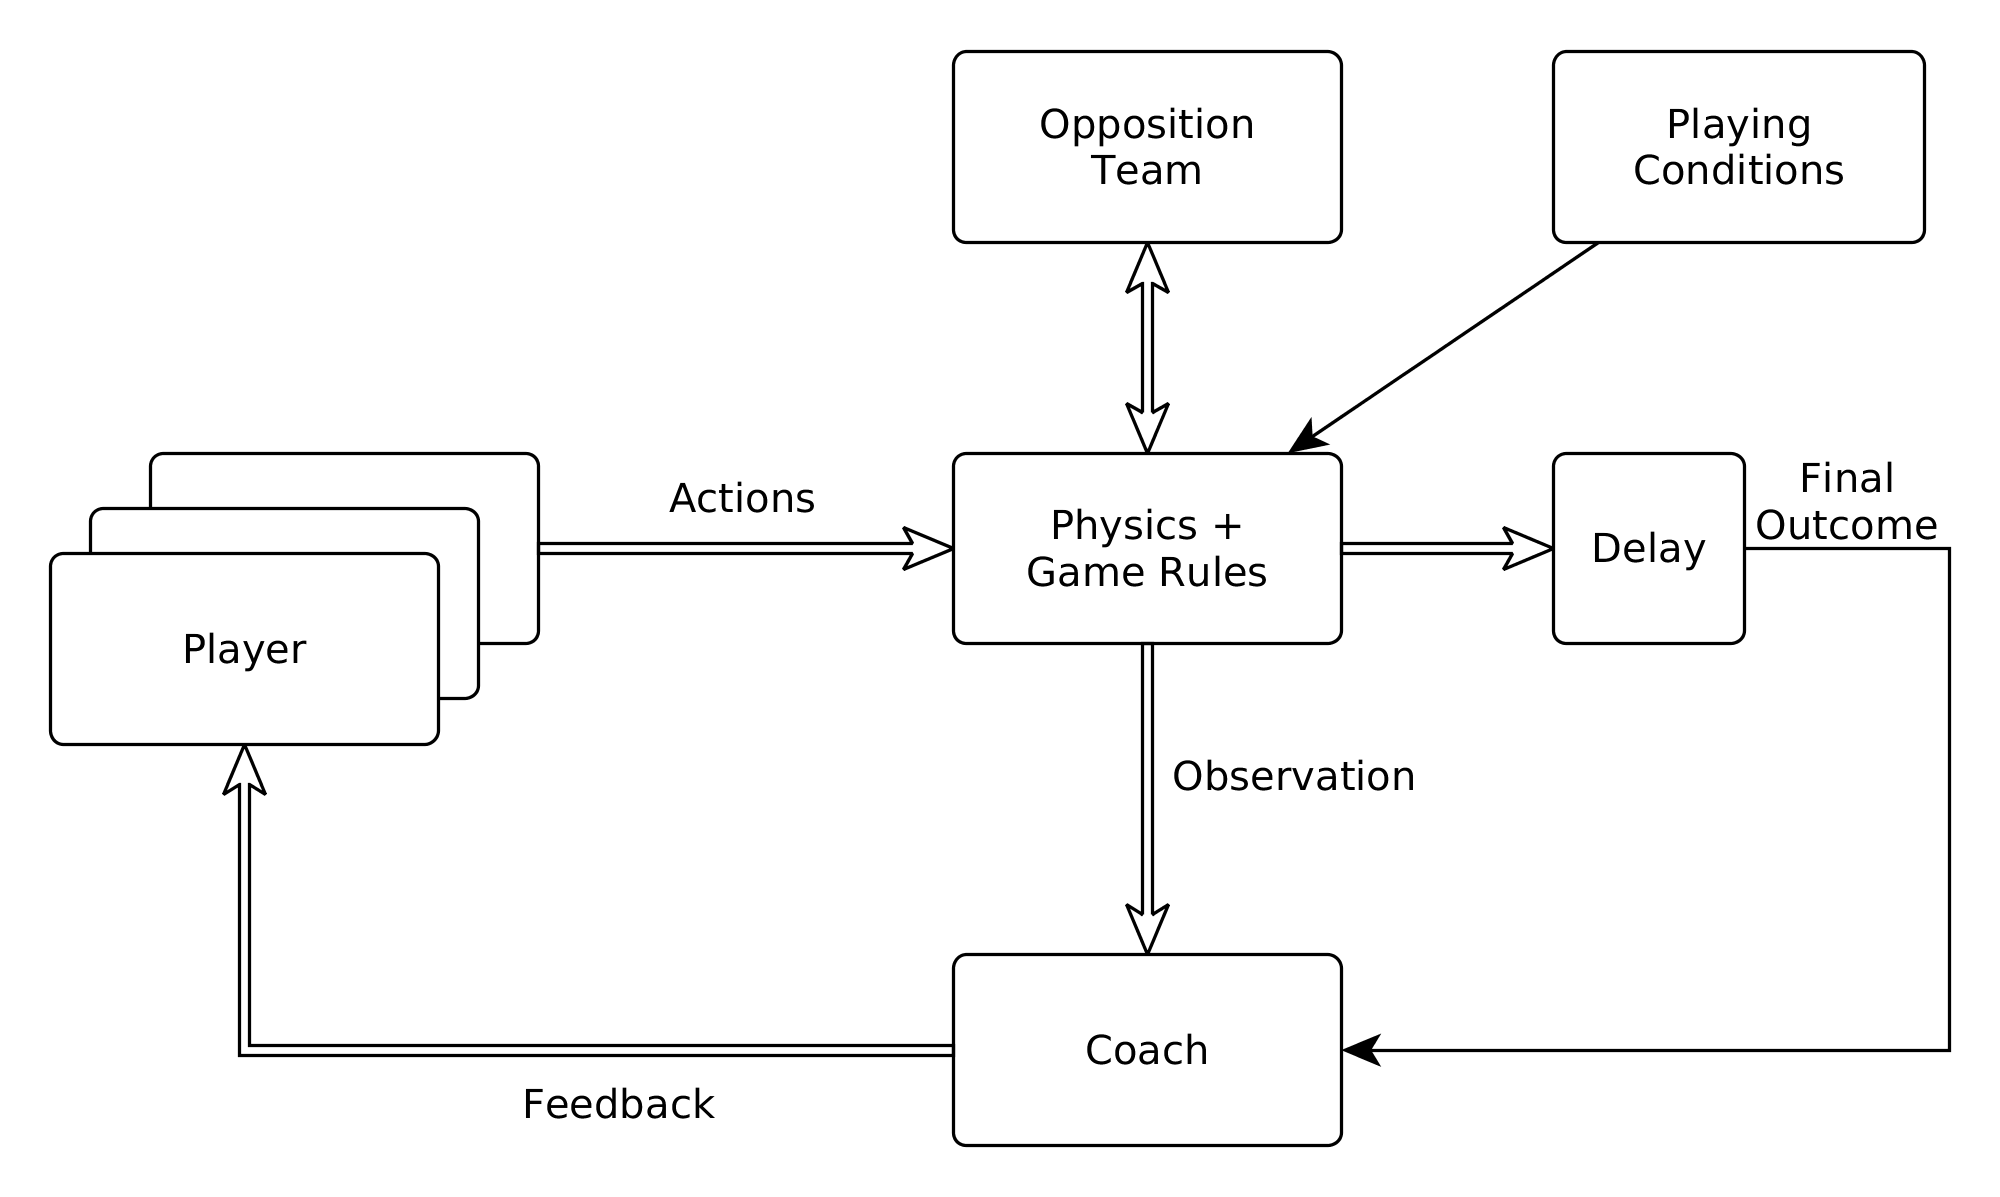
\includegraphics[width=\linewidth]{figs/model/feedback_model.png}
\caption{Feedback Model \label{fig:feedback}}
\end{figure}

% Associate supervisor suggested "transform it into feedback for the players to action".
% -> Reject (feedback is not commands, it is up to players to decide how to convert feedback to actions)
% -> Never mind, accepted.
Ultimately, the information a coach has access to is only useful if the
coach can transform it into feedback for the players to action.
A feedback model was developed to analyse feedback information flows available in competitive team sport, which is presented in \figref{fig:feedback}, and described in greater detail below.
% This model is described in greater detail below.

% The game is between two teams, coordinated by the coaches. However,
% economic theory and organizational behavior theory highlight the
% need to also consider the motivations of the individual players.
% We model the
% individual players as agents that seek to optimize their action
% selection so as to maximize the expected reward signal in the feedback
% received from the coaches.
% It is important that the coach carefully
% select the player reward signal such that it will cause the players to
% select actions that align with the coach's objective of winning games.
% The best way to achieve this is to ensure that the player reward signal
% aligns with the actual value delivered to the team. The coach also needs
% to take into account the way that players learn behavior - this allows
% the coach to design a feedback system that maximizes the player's
% learning so that the player can quickly achieve peak performance.

Players select actions based upon the context of the situation they are
presented with. The actions of both teams combine through the laws of
physics, as well as the laws of the game enforced by the umpires, to
result in a concrete outcome, such as a goal scored. The outcome is the
combined result of all players. Lames and
McGarry \cite{lames2007search} discuss how this interaction process is so involved that the
underlying skill is not observable through a traditional approach, and
go so far as to suggest that performance analysis in team sport is so
difficult that it requires a qualitative methodology. Player actions can be observed, however their consequences are not always directly apparent (e.g. a strategic pass may at first appear a poor decision, but later lead to the team scoring a goal). This is represented in the feedback model as a ``Delay'' between when the player actions take place, and the final game outcome.

``Playing Conditions'' is also included in the diagram to represent
the weather and ground conditions that introduce unpredictable
variations into the game. Although the laws of physics (to a classical
mechanics approximation) are deterministic in principle, small
unmeasurable variations of weather and the playing surface can cause the
ball to bounce in a different direction, and ultimately affect the final
outcome of the game. Thus, for all practical purposes, the
game is a stochastic process \cite{Forbes2006}.

For long term optimisation over many games, coaches could feed back the
final game outcome to the players as a way of training them how to
improve. However, this is not practical as the sole source of feedback, as players would
need to experiment over many games to identify the underlying cause of performance issues. Furthermore, it is not clear
how the coach should assign credit to individual player actions, as the
final outcome is a result of many actions combined.

Instead, the coach uses their observations of the game along with statistics provided by sport performance analysts in order to provide players with more direct feedback that reflects how the coach believes player actions
contribute to the final game outcome. This form of feedback is more immediate and actionable than game outcomes alone, as it tries to explain performance rather than just measure performance. However, it can be compromised in three ways: inaccurate observations of the game state, feeding back a measure that does not align with overall team
performance, or not accounting for the psychology of the way players
learn from feedback.

\section{Information Theoretic Perspective}
\label{sec:info-theory-perspective}

This section explains how information theory can provide the field of sport
science with rigorous answers to the following questions, which were
previously only answerable based upon the anecdotal experiences of
sport scientists and coaches: \emph{What is the purpose of transforming
and summarising sport data if it cannot create new information beyond
what coaches can manually observe by watching the game? What value does
interactive data analysis offer over pre-defined analysis procedures?}

In a single player sport such as archery, performance is easily
observable through game outcomes. Whilst there is an element of luck
involved, this can be eliminated by averaging outcomes over multiple
attempts. In contrast, measuring performance in team sport is an
intractable problem, as the game outcome is the result of many players'
interactions. Furthermore, even a minor disturbance, such as a gust of
wind, could influence the game outcome. These issues led Lames and
McGarry \cite{lames2007search} to declare classical quantitative
performance indicators unreliable measures of team sport. To address
this failure, Lames and McGarry speculate upon the possibility of
modelling sport as a complex system, although they suggest that a qualitative
approach may be more practical.

This section analyses the flow of information in team sport performance measurement from an information theoretic
\cite{Shannon1948} perspective, which provides a
mathematical framework for rigorously reasoning about information flows.
Unlike Lames and McGarry, it does not dismiss quantitative team
performance measurement as unreliable based upon the perceived
complexity of team interactions; instead, it uses information theory to
reason about the theoretical limits of such an approach. Note that qualitative approaches also constitute a form of information flow that must also obey information theoretic constraints,
albeit harder to accurately measure.

\subsection{Problem Formalisation}\label{problem-formalization}

The information flow diagram depicted in Shannon's
original paper on information theory, \textit{A Mathematical Theory of Communication} \cite{Shannon1948}, was adapted for the sport domain. The adaptation includes game interaction process described by Lames and McGarry \cite{lames2007search}, sensing, automated analysis,
as well as a
simplified model to represent the cognitive interpretation of visual
information. The resultant information flows for performance analysis in
sport are depicted in \figref{fig:measure-interpret}.

\begin{landscape}

\begin{figure}[htbp]
\centering
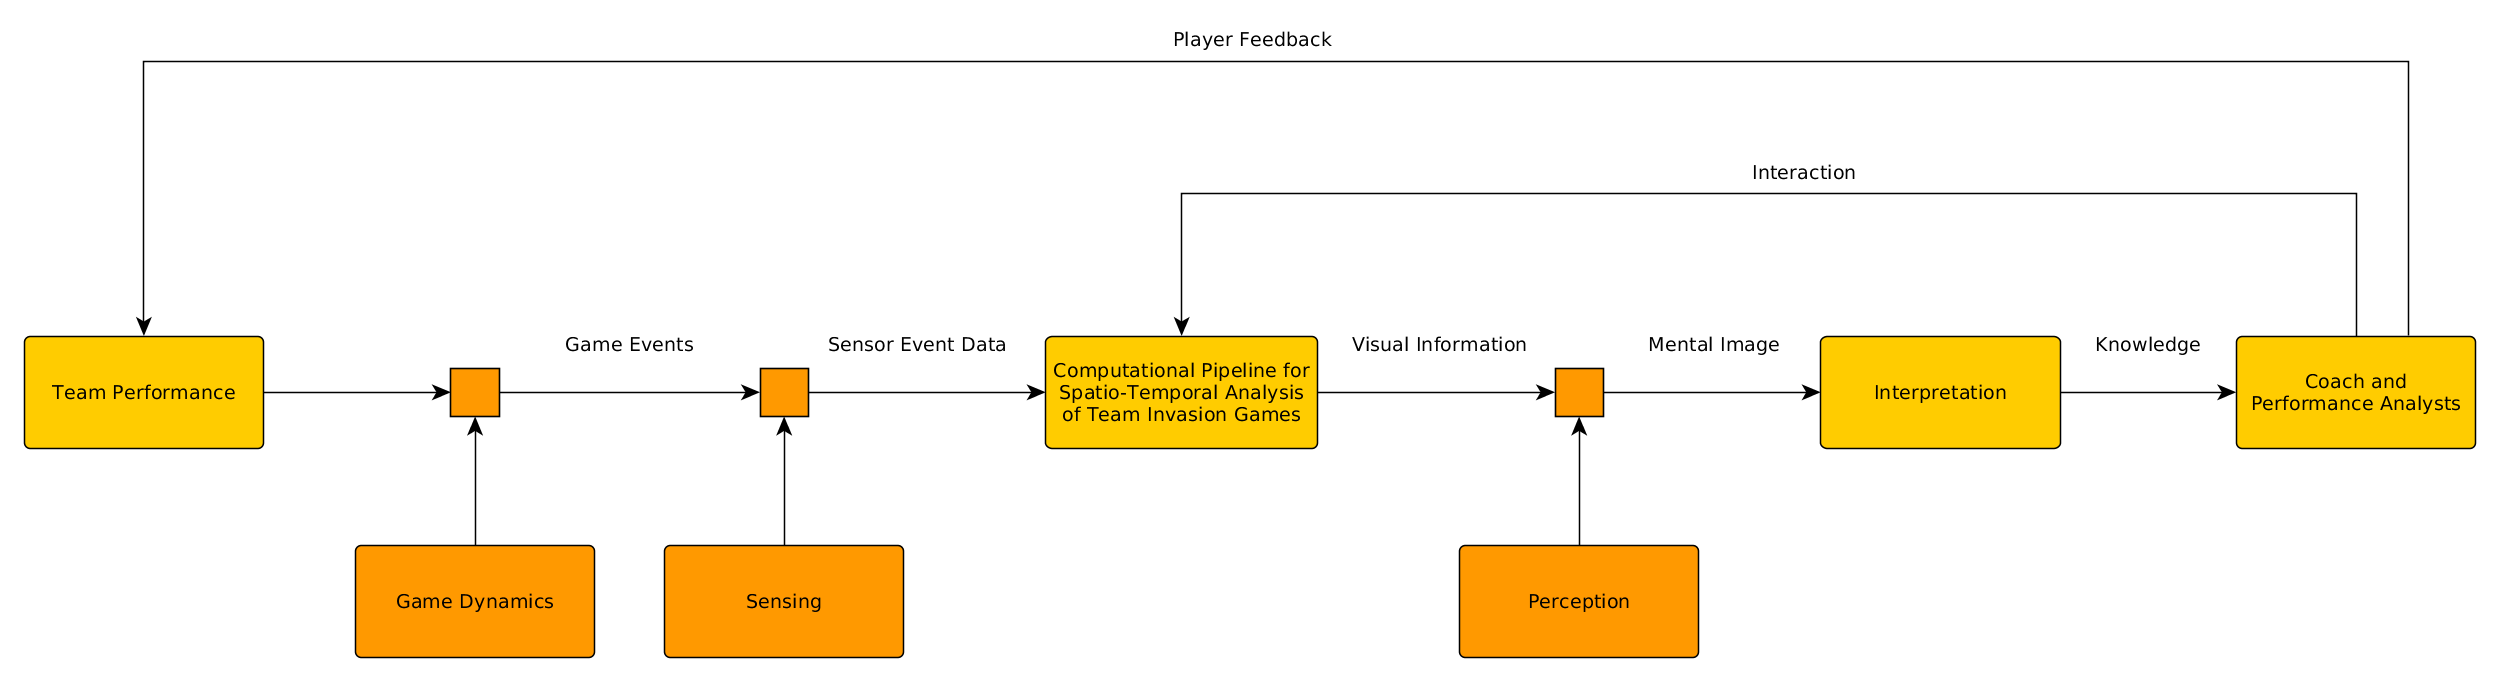
\includegraphics[width=\linewidth]{measure-interpret.png}
\caption{Information Flow in Performance Measurement Process
\label{fig:measure-interpret}}
\end{figure}

\end{landscape}

\begin{minipage}{1.0\textwidth}
The chain of processes involved (other than coaching interaction with the computational pipeline, which will be discussed later in \secref{sec:infotheory-discussion}) is represented mathematically as:

\[Know = (Interp \circ Percep \circ Comp \circ Sens \circ Dyn) (Perf)\]


Where:
\begin{description}
    \item[$f \circ g$] represents function composition of two arbitrary functions $f$ and $g$. i.e. $f \circ g = f(g(...))$
    \item[$Perf$] is the team performance. This incorporates the individual skills, abilities, and decision making of each player, as well as team factors such as team playing style, and team cohesion.
    \item[$Dyn$] is a function representing the game dynamics that captures how individual player interactions become game events.
    \item[$Sens$] is a function representing the sensor observations of the game, and any noise introduced by imperfect sensors.
    \item[$Comp$] is the function implemented by the computational pipeline that analyses sensor inputs and outputs game information for visual display to the coach and performance analysts. The computational pipeline may contain many sub-components; however, together they are still only one component of the overall sport performance measurement and feedback process.
    \item[$Percep$] is a function representing the coach's ability to perceive visual information, taking into account visual acuity.
    \item[$Interp$] is a function representing the coach's interpretation of the visualisation, transforming a visual representation of the game into knowledge about the game.
    \item[$Know$] is the knowledge of the game delivered to the coach by the system. This is defined to include both trivial facts about players, as well as deeper knowledge about the game itself that helps the coach to predict the results of actions within the game.
\end{description}
\end{minipage}

\vspace{1em}

The aim of a computational pipeline for sport performance analysis is to give the coach greater knowledge of team performance. This can be formalised in terms of information entropy. Specifically, by looking at the amount of information about team performance that remains unknown to the coach. From this perspective, the aim of the computational pipeline is to produce a visualisation that reduces the amount of unknown information about team performance.

Formally this can be stated as: given prior knowledge of the sport domain,
find a pair of functions for \emph{Computation} and \emph{Interpretation}, which minimise the entropy of \emph{Team Performance} conditional upon the \emph{knowledge delivered
to the coach}.

\[\min_{Comp, Interp} H(Perf|Know)\]

\begin{minipage}{1.0\textwidth}
Where:
\begin{description}
    \item[$H$] is information entropy, as defined by Shannon \cite{Shannon1948}.
    \item[$Perf$] represents the team performance of interest to coaches as defined earlier.
    \item[$Know$] is the coach's knowledge of team performance as defined earlier, enhanced via computations $Comp$ interpreted according to $Interp$ delivered via the chain of (noisy) processes described earlier.
\end{description}
\end{minipage}

%\subsection{Heuristic Solutions}\label{heuristic-solutions}

\subsection{Theoretical Solution}\label{heuristic-solution-1}

If the intermediate distortion functions were reversible, then it would be possible to
find an optimal solution. The components of an ideal performance analysis pipeline, and its interpretation are depicted in \figref{fig:soln1-inverse}.

\begin{figure}[htbp]
\centering
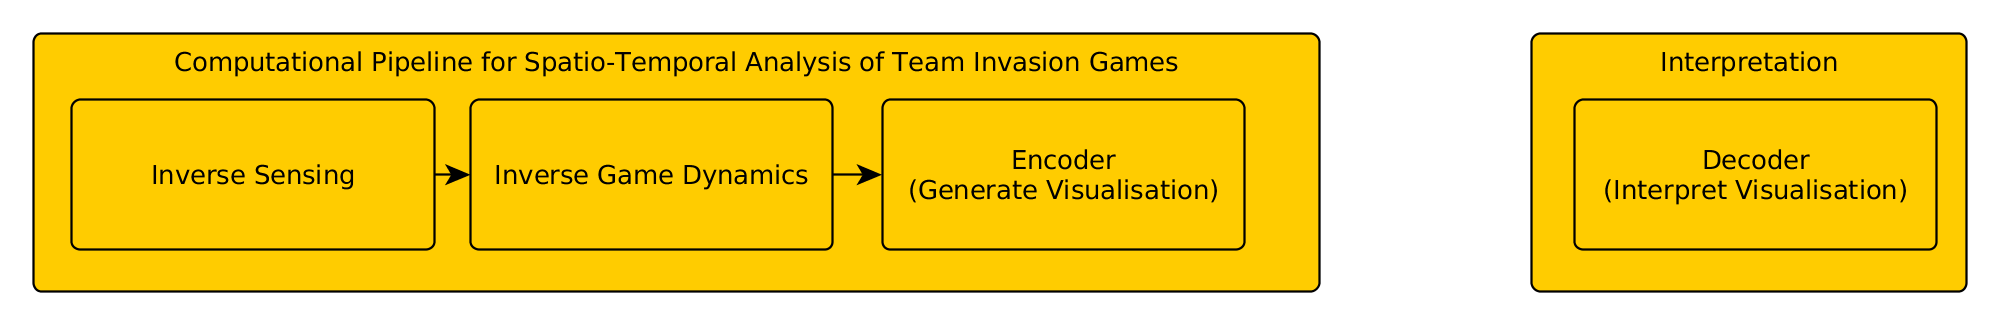
\includegraphics[width=\linewidth]{soln1-inverse.png}
\caption{Theoretical Solution: Inverse distortions. \label{fig:soln1-inverse}}
\end{figure}

Theoretically, one could invert the sensor readings to obtain the game events, and
then invert the game dynamics in order to find the underlying team
performance. As sensor technologies improve, inverting the sensor data
to obtain the game data is becoming feasible. Historically, only a small
number of events were captured in sport games, such as the total number
of goals scored by each player. This discards much of the game
information (such as the time the goals were scored), thus making an
exact reconstruction of the game impossible. With the development of
pervasive sensing technologies for sport that can track players' every movement, near-exact reconstruction of game events from sensor data is now possible.

%\footnote{Catapult Sports, ``Catapult
%  OptimEye''. http://www.catapultsports.com/au/system/outdoor/
%  Accessed:2017-03-20} \footnote{Catapult Sports, ``Catapult ClearSky''.
%  http://www.catapultsports.com/au/system/indoor/ Accessed:2017-03-20}
%\footnote{STATS, ``STATS SportVu basketball player tracking''.
%  https://www.stats.com/sportvu-basketball/ Accessed:2017-03-20}

The challenge, however, lies in inverting the game dynamics to obtain
the team performance from game events. In strategic games, such as
backgammon, it is possible to evaluate human decisions by comparing to
the ideal choice determined by computer simulation
\cite{oshaughnessy_identification_2016}. Whilst AI players can
dominate humans in abstract strategy games such as backgammon, chess, and Go \cite{silver2016mastering}, AI controlled sport players\footnote{RoboCup
  Federation, ``A Brief History of RoboCup''.
  http://www.robocup.org/a\_brief\_history\_of\_robocup
  Accessed:~2017-03-20} are yet to master basic skills within physical
environments. As such, there is no reliable ``optimal'' decision to
evaluate players against, implying that precisely inverting the game
dynamics function is not yet possible.

However, heuristics exist to approximate the inversion so as to obtain
performance from game events. For example, \afl{}
equity ratings \cite{Jackson2016} examine the contribution a player makes to their
team based upon the changes they make to the expected score. Note that
the current AFL equity rating only considers factors such as
team-with-possession and position-of-ball, and discards consideration of
players without the ball in the estimation of expected score, so is
clearly a heuristic rather than a precise measure of a player's true
contribution.

If both game dynamics and sensing could be accurately inverted, then team
performance could be recovered precisely. At this point, transmitting the
team performance to the coach would simply be a matter of encoding the
performance results, either numerically or visually, for the coach to
interpret.

Shannon's mathematical theory of communications
\cite{Shannon1948} reveals that this information can in
theory be transmitted to the coach more effectively by designing an
encoding structure that takes advantage of the known properties of the
performance signal. For example, if the performance is usually ``player
1: normal, player 2: normal, \ldots{}'', then one could create a simple
symbol to represent all-players-are-normal-performance, and devise more
complex symbols to represent anomalous situations that rarely occur.
However, interpretation of visualisations requires cognitive resources which are likely to outweigh
any information-capacity benefits attained through compressing data
using complex visual encoding schemes. In practice, it is well
established in the information visualisation literature that visual
encoding should cater to address the limits of human cognition rather
than maximum information density \cite{Anderson2011, Huang2009}. This can potentially be achieved using a framework such as Physics of Notations
\cite{Moody2009}.

%\subsubsection{Heuristic Solution}\label{heuristic-solution-2}
\subsection{Heuristic Solution}\label{sec:heuristic-solution-2}

An alternative option that bypasses the need to build a full model of
the game is to extract features that correlate with performance. Ideally
the features selected for display to the coach should be independent of
each other, as a set of features that correlate with each other would
contain redundant information that makes inefficient use of both space
on the visualisation, as well as the coach's cognitive resources to
process this information. The components of this heuristic solution are
depicted in \figref{fig:soln2-pca}.

\begin{figure}[htbp]
\centering
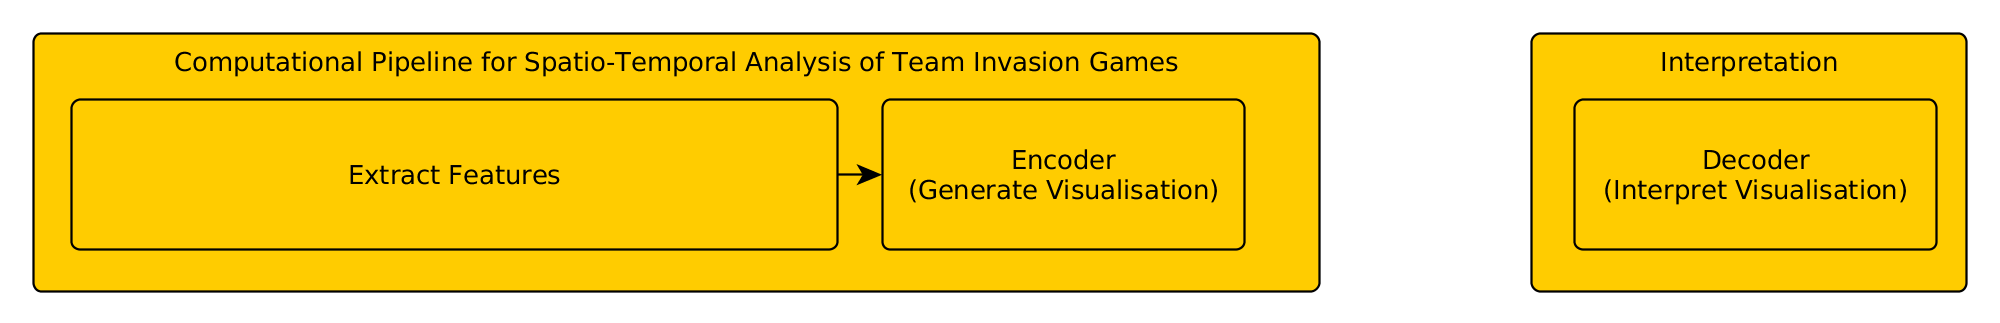
\includegraphics[width=\linewidth]{soln2-pca.png}
\caption{Heuristic Solution: Extract features \label{fig:soln2-pca}}
\end{figure}

A simple algorithm for creating such a set of independent features is
Principal Component Analysis (PCA). Note however, that Principal
Component Analysis is linear, so will not be able to detect team
performance features that aren't revealed as simple linear combinations
of sensor features. This heuristic can be enhanced by first transforming
the sensor space into a domain where combinations of sensor features are
more likely to correlate linearly with team performance. For example,
player agility may not be obvious from player position recordings alone,
but might become obvious once transformed to frequency space using a
Fourier transform, thus revealing periodic movements---which might be
generated by movements such as swerving between players---as components
of the spectrum.

As with the theoretical approach, these derived features are then presented to
the coach. The coach may interact with the system in order to select the
features that they believe provide the highest information content. This
interaction allows the coach to improve the efficiency of the encoding
by filtering out signals that do not correlate well with team
performance, as well as allowing them to removing unsurprising features
that reveal aspects of team performance that they were already well
aware of (e.g.~from their manual observations of the game).

\subsection{Discussion}\label{sec:infotheory-discussion}

By viewing sport analysis through the lens of information theory, it is possible to draw answers to the questions set out at the start of this section of the thesis.

\subsubsection{What is the purpose of transforming
and summarising sport data if it cannot create new information beyond
what was present in the raw
dataset?}

If the coach had unlimited cognitive resources, then computational pipelines, from an information theoretic perspective, can not offer any
additional value beyond what is present in the raw dataset, as they
cannot generate new information in an information theoretic sense.
However, in practice, the capacity of the coach's cognition channels are
limited. The psychological phenomenon of ``inattentional
blindness'' \cite{Simons1999} shows that humans do not have the ability to
reliably monitor all player interactions simultaneously. As such, the
purpose of a sport data analysis pipeline is to extract the features of the game
that provide the highest information content about team performance, and
filter irrelevant information, thus maximising the value of information
transferred over the coach's limited cognitive channels.

\subsubsection{What value does interactive data
analysis offer over pre-defined analysis
procedures?}

As outlined in the Heuristic Solution (\secref{sec:heuristic-solution-2}), interaction provides the ability
for the coach to customise the data analysis to
provide them with information they don't already know. Minimising the
entropy $H(Perf|Know)$ requires information that is independent of the
coach's prior knowledge of performance.

\subsection{Limitations}\label{limitations}

Team performance was defined to incorporate the
individual skills, abilities, and decision making of each player, as
well as team factors such as team playing style, and team cohesion.
However, it is unclear how this should be represented. It is also
unclear whether it is possible to quantify individual performance
rigorously within the context of a team. The mathematical field of
``game theory''\footnote{Wikipedia Contributors, ``Game theory''.
  https://en.wikipedia.org/wiki/Game\_theory Accessed:~2017-03-20} shows
many problematic scenarios where maximising individual utility functions
does not maximise net utility for the team, which may undermine
incentive schemes designed to reward players for individual performance.

% Associate supervisor thinks this should be highlighted earlier in intro
Through an information theoretic lens, the main constraint on the processing was considered to be the information capacity limit on the coach's ability to perceive
information. In practice, an additional constraint is the coach's speed
of mental computation. Even if a coach has access to all the knowledge
that they need to accurately determine performance in theory, it's
possible that the knowledge is in a form such that computing the
performance from the knowledge could take excessive amounts of
computation, well beyond what a human is capable of. In future, the model could be extended to include mental computation constraints by combining the information theoretic perspective used to analyse information capacity constraints with a cognitive load perspective to analyse the mental computation constraints.

% Finally, while it sounds reasonable to assume that the role of a sport performance analysis system is to gain knowledge of team performance,
% some may debate this. A more holistic view is that the aim of a
% sport performance analysis system is to allow the coach to provide player
% feedback. This could be partially addressed in the proposed system by redefining the
% team performance variable to be the aspects of team performance
% requiring feedback.

%\nb{Tie back to "exploration versus exploitation" concept in reinforcement learning}

\subsection{Conclusion}\label{conclusion-infotheory}

Using an information theoretic framework, this section of the thesis showed that computational pipelines have a clear role to play in the sport coaching
process, as a tool to provide coaches with the most important
information required to enhance their knowledge of the game. Conventional performance
indicators such as ``number of kicks'' are unlikely to offer the coach
any useful information, as this is something that the coach will already
have approximate knowledge of from their manual observations of the
game. Instead, the proposed model suggests that sport performance analysis systems should
focus on providing information that the coach has minimal prior
knowledge of.

%It should
%be noted however, that existing systems designed without the proposed model do
%not necessarily achieve this aim.

Future work is needed to devise measures for each attribute, and
approximations of each function, in order to provide numerical
estimates of the information gain offered by incorporating analysis tools into the sport performance process (this is a non-trivial task as it requires both functions to
simulate the game, as well as functions to approximate the coach's
cognition). Another area to explore is to model the feedback
as part of a learning system where the goal is not knowledge of any
individual signal, but rather stability of the overall system---possibly deliberately taking sub-optimal actions in order to learn from them (the human equivalent of the exploration-exploitation trade-off faced by autonomous agents in the field of reinforcement learning \cite{sutton1998reinforcement}). As future work, it is also necessary to incorporate computation limits into the proposed model. However, even as stands, the model provided is capable of providing a new
perspective on the value of computational pipelines within the larger sport performance feedback process.
